\documentclass[a4paper,12pt]{mwart}
\usepackage{graphicx}
\usepackage{amsmath,amsfonts,amsthm,amssymb,mathtools}
\usepackage{polski}
\begin{document}
    \title{Dokumentacja}

\maketitle
\section{Schemat bazy danych}
\begin{figure}[h!]
    \centering

    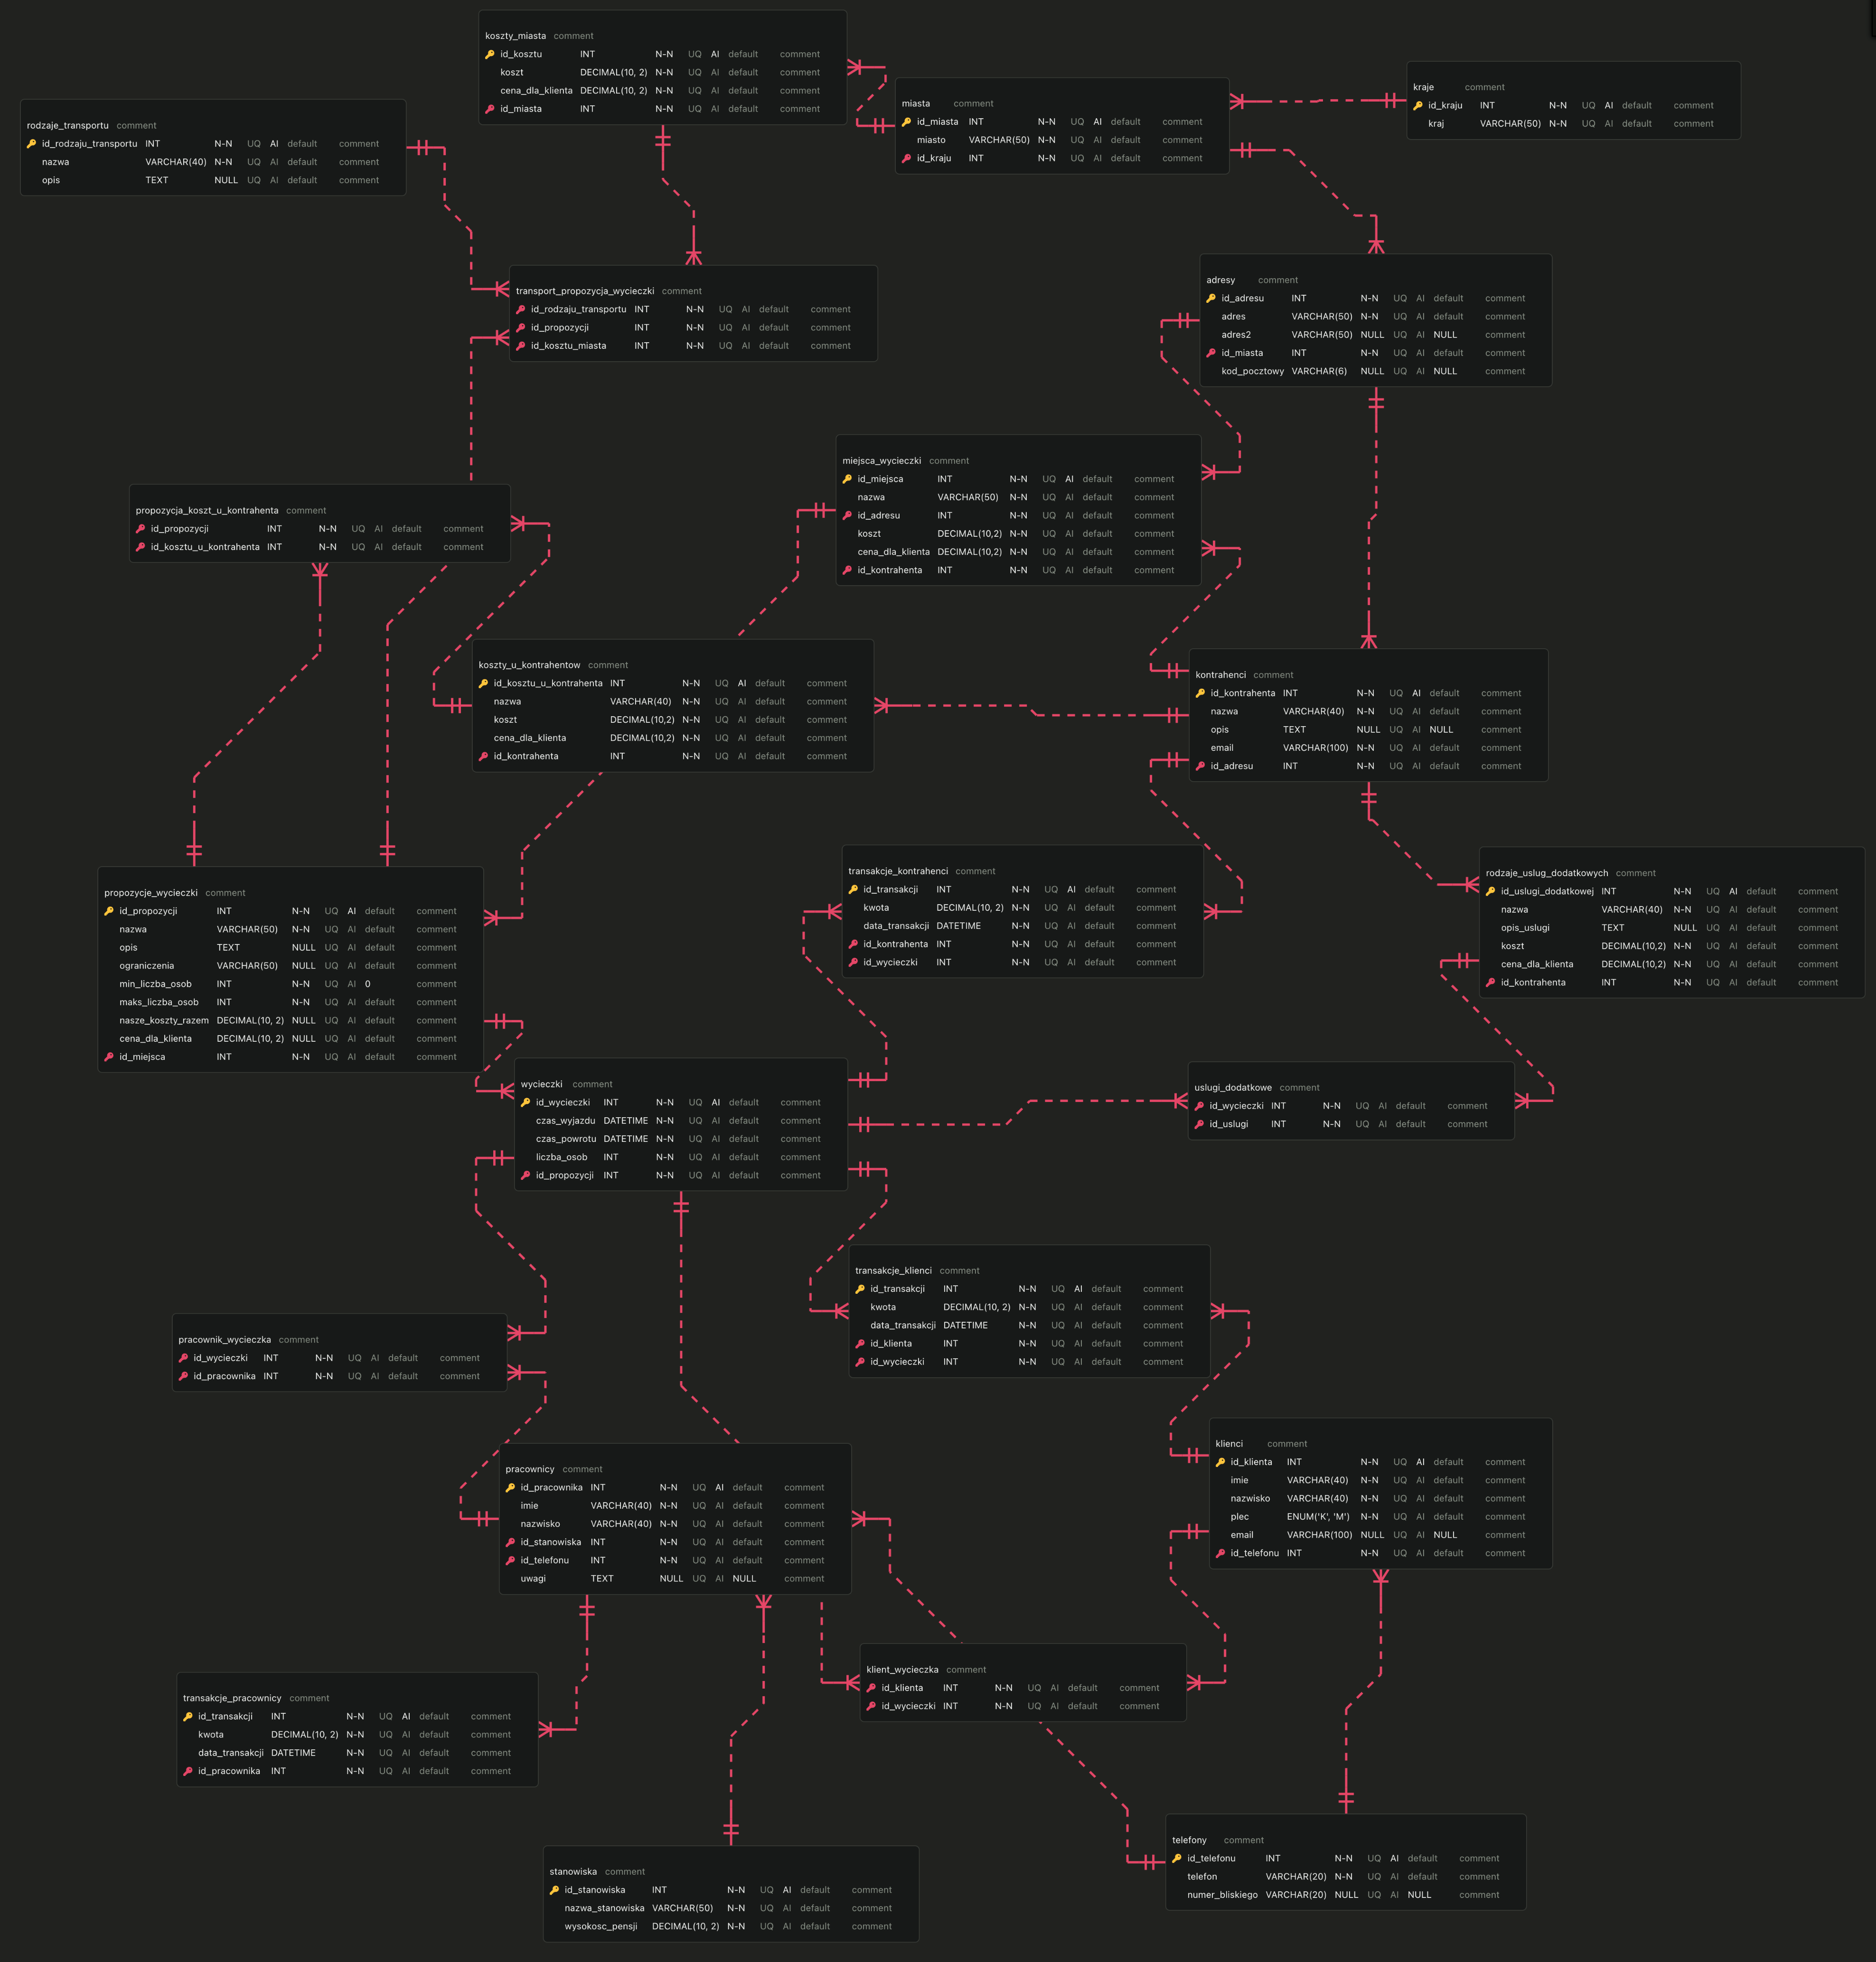
\includegraphics[scale=0.1]{../obrazy/baza_danych_fullsize.png}
    \caption{Schemat bazy danych}
\end{figure}
\section{Analiza tabel}
\subsection{Tabela rodzaje\_transportu}
Tabela jest postaci:

rodzaje\_transportu(\underline{id\_rodzaju\_transportu}, nazwa, opis)

\noindent Jedynymi nietrywialnymi zależnościami funkcyjnymi są:
$$   id\_rodzaju\_transportu  \rightarrow nazwa $$
$$   id\_rodzaju\_transportu  \rightarrow opis$$
Zatem każda nietrywialna zależność funkcyjna zaczyna się od nadklucza i tabela  spełnia wymagania bycia w EKNF.

\subsection{Tabela koszty\_miasta}
Tabela jest postaci:

koszty\_miasta(\underline{id\_kosztu\_miasta}, koszt, cena\_dla\_klienta, id\_miasta)

\noindent Jedynymi nietrywialnymi zależnościami funkcyjnymi są:
$$   id\_kosztu\_miasta  \rightarrow koszt $$
$$   id\_kosztu\_miasta  \rightarrow cena\_dla\_klienta $$
$$   id\_kosztu\_miasta  \rightarrow id\_miasta $$

Zatem każda nietrywialna zależność funkcyjna zaczyna się od nadklucza i tabela  spełnia wymagania bycia w EKNF.

\subsection{Tabela miasta}
Tabela jest postaci:

miasta(\underline{id\_miasta}, miasto, id\_kraju)

\noindent Jedynymi nietrywialnymi zależnościami funkcyjnymi są:
$$   id\_miasta  \rightarrow miasto $$
$$   id\_miasta  \rightarrow id\_kraju $$
Zakładamy, że miasto nie definiuje jednoznacznie kraju.
Zatem każda nietrywialna zależność funkcyjna zaczyna się od nadklucza i tabela  spełnia wymagania bycia w EKNF.

\subsection{Tabela kraje}
Tabela jest postaci:

kraje(\underline{id\_kraju}, kraj)

\noindent Jedyną nietrywialną zależnością funkcyjną jest:
$$   id\_kraju  \rightarrow kraj$$


Zatem każda nietrywialna zależność funkcyjna zaczyna się od nadklucza i tabela  spełnia wymagania bycia w EKNF.

\subsection{Tabela transport\_propozycja\_wycieczki}
Tabela jest postaci:

transport\_propozycja\_wycieczki(id\_rodzaju\_transportu, id\_propozycji, id\_kosztu\_miasta)

W tej tabeli nie występują nietrywialne zależności funkcyjne, wszystkie trzy kolumny tworzą klucz elementarny, a pomiędzy nimi nie ma zależności.
Zatem każda nietrywialna zależność funkcyjna zaczyna się od nadklucza i tabela  spełnia wymagania bycia w EKNF.

\subsection{Tabela adresy}
Tabela jest postaci:

adresy(\underline{id\_adresu}, adres, adres2, id\_miasta, kod\_pocztowy)

\noindent Jedynymi nietrywialnymi zależnościami funkcyjnymi są:
$$   id\_adresu  \rightarrow adres $$
$$   id\_adresu  \rightarrow adres2 $$
$$   id\_adresu  \rightarrow id\_miasta $$
$$   id\_adresu  \rightarrow kod\_pocztowy $$
Zakładamy, że kod pocztowy nie definiuje jednoznacznie miasta i  adres nie definiuje kodu pocztowego.


Zatem każda nietrywialna zależność funkcyjna zaczyna się od nadklucza i tabela  spełnia wymagania bycia w EKNF.


\subsection{Tabela miejsca\_wycieczki}
Tabela jest postaci:

miejsca\_wycieczki(\underline{id\_miejsca}, nazwa, id\_adresu, koszt, cena\_dla\_klienta, id\_kontrahenta)

\noindent Jedynymi nietrywialnymi zależnościami funkcyjnymi są:
$$   id\_miejsca  \rightarrow nazwa $$
$$   id\_miejsca  \rightarrow id\_adresu $$
$$   id\_miejsca  \rightarrow koszt $$
$$   id\_miejsca  \rightarrow cena\_dla\_klienta $$
$$   id\_miejsca  \rightarrow id\_kontrahenta $$


Zatem każda nietrywialna zależność funkcyjna zaczyna się od nadklucza i tabela  spełnia wymagania bycia w EKNF.

\subsection{Tabela propozycja\_koszt\_u\_kontrahenta}
Tabela jest postaci:

propozycja\_koszt\_u\_kontrahenta(id\_propozycji, id\_kosztu\_u\_kontrahenta)

W tej tabeli nie występują nietrywialne zależności funkcyjne, wszystkie trzy kolumny tworzą klucz elementarny, a pomiędzy nimi nie ma zależności.
Zatem każda nietrywialna zależność funkcyjna zaczyna się od nadklucza i tabela  spełnia wymagania bycia w EKNF.


\subsection{Tabela koszty\_u\_kontrahenta}
Tabela jest postaci:

koszty\_u\_kontrahenta(\underline{id\_kosztu\_u\_kontrahenta}, nazwa, koszt, cena\_dla\_klienta, id\_kontrahenta)

\noindent Jedynymi nietrywialnymi zależnościami funkcyjnymi są:
$$   id\_kosztu\_u\_kontrahenta\rightarrow nazwa $$
$$   id\_kosztu\_u\_kontrahenta\rightarrow koszt $$
$$   id\_kosztu\_u\_kontrahenta\rightarrow cena\_dla\_klienta $$
$$   id\_kosztu\_u\_kontrahenta\rightarrow id\_kontrahenta $$


Zatem każda nietrywialna zależność funkcyjna zaczyna się od nadklucza i tabela  spełnia wymagania bycia w EKNF.


\subsection{Tabela kontrahenci}
Tabela jest postaci:

kontrahenci(\underline{id\_kontrahenta}, nazwa, opis, email, id\_adresu)

\noindent Jedynymi nietrywialnymi zależnościami funkcyjnymi są:
$$   id\_kontrahenta  \rightarrow nazwa $$
$$   id\_kontrahenta  \rightarrow opis $$
$$   id\_kontrahenta \rightarrow email $$
$$   id\_kontrahenta \rightarrow id\_adresu $$


Zatem każda nietrywialna zależność funkcyjna zaczyna się od nadklucza i tabela  spełnia wymagania bycia w EKNF.


\subsection{Tabela propozycje\_wycieczki}
Tabela jest postaci:

propozycje\_wycieczki(\underline{id\_propozycji}, nazwa, opis, ograniczenia, min\_liczba\_osob, max\_liczba\_osob, nasze\_koszty\_razem, cena\_dla\_klienta, id\_miejsca)

\noindent Jedynymi nietrywialnymi zależnościami funkcyjnymi są:
$$   id\_propozycji  \rightarrow nazwa $$
$$   id\_propozycji\rightarrow opis $$
$$   id\_propozycji\rightarrow ograniczenia $$
$$   id\_propozycji\rightarrow min\_liczba\_osob $$
$$   id\_propozycji\rightarrow max\_liczba\_osob $$
$$   id\_propozycji\rightarrow nasze\_koszty\_razem $$
$$   id\_propozycji\rightarrow cena\_dla\_klienta $$
$$   id\_propozycji\rightarrow id\_miejsca $$


Zatem każda nietrywialna zależność funkcyjna zaczyna się od nadklucza i tabela  spełnia wymagania bycia w EKNF.

\subsection{Tabela wycieczki}
Tabela jest postaci:

wycieczki(\underline{id\_wycieczki}, czas\_wyjazdu, czas\_powrotu, liczba\_osob, id\_propozycji)

\noindent Jedynymi nietrywialnymi zależnościami funkcyjnymi są:
$$   id\_wycieczki\rightarrow czas\_wyjazdu$$
$$   id\_wycieczki\rightarrow czas\_powrotu $$
$$   id\_wycieczki\rightarrow liczba\_osob $$
$$   id\_wycieczki\rightarrow id\_propozycji $$


Zatem każda nietrywialna zależność funkcyjna zaczyna się od nadklucza i tabela  spełnia wymagania bycia w EKNF.

\subsection{Tabela transakcje\_kontrahenci}
Tabela jest postaci:

transakcje\_kontrahenci(\underline{id\_transakcji}, kwota, data\_transakcji, id\_kontrahenta, id\_wycieczki)

\noindent Jedynymi nietrywialnymi zależnościami funkcyjnymi są:
$$   id\_transakcji\rightarrow kwota $$
$$   id\_transakcji\rightarrow czas\_wyjazdu$$
$$   id\_transakcji\rightarrow data\_transakcji $$
$$   id\_transakcji\rightarrow id\_kontrahenta $$
$$   id\_transakcji\rightarrow id\_wycieczki$$

Zatem każda nietrywialna zależność funkcyjna zaczyna się od nadklucza i tabela  spełnia wymagania bycia w EKNF.

\subsection{Tabela rodzaje\_uslug\_dodatkowych}
Tabela jest postaci:

 rodzaje\_uslug\_dodatkowych(\underline{id\_uslugi\_dodatkowej}, nazwa, opis\_uslugi, koszt, cena\_dla\_klienta, id\_kontrahenta)

\noindent Jedynymi nietrywialnymi zależnościami funkcyjnymi są:
$$   id\_uslugi\_dodatkowej\rightarrow nazwa $$
$$   id\_uslugi\_dodatkowej\rightarrow opis\_uslugi$$
$$   id\_uslugi\_dodatkowej\rightarrow koszt$$
$$   id\_uslugi\_dodatkowej\rightarrow cena\_dla\_klienta $$
$$   id\_uslugi\_dodatkowej\rightarrow id\_kontrahenta$$

Zatem każda nietrywialna zależność funkcyjna zaczyna się od nadklucza i tabela  spełnia wymagania bycia w EKNF.


\subsection{Tabela uslugi\_dodatkowe}
Tabela jest postaci:

uslugi\_dodatkowe(id\_wycieczki, id\_uslugi)

W tej tabeli nie występują nietrywialne zależności funkcyjne, dwie kolumny  tworzą klucz elementarny, a pomiędzy nimi nie ma zależności.
Zatem każda nietrywialna zależność funkcyjna zaczyna się od nadklucza i tabela  spełnia wymagania bycia w EKNF.

\subsection{Tabela pracownik\_wycieczka}
Tabela jest postaci:

pracownik\_wycieczka(id\_wycieczki, id\_pracownika)

W tej tabeli nie występują nietrywialne zależności funkcyjne, dwie kolumny  tworzą klucz elementarny, a pomiędzy nimi nie ma zależności.
Zatem każda nietrywialna zależność funkcyjna zaczyna się od nadklucza i tabela  spełnia wymagania bycia w EKNF.

\subsection{Tabela pracownicy}
Tabela jest postaci:

pracownicy(\underline{id\_pracownika}, imie, nazwisko, id\_stanowiska, id\_telefonu, uwagi)

\noindent Jedynymi nietrywialnymi zależnościami funkcyjnymi są:
$$   id\_pracownika\rightarrow imie $$
$$   id\_pracownika\rightarrow nazwisko $$
$$   id\_pracownika\rightarrow id\_stanowiska $$
$$   id\_pracownika\rightarrow id\_telefonu $$
$$   id\_pracownika\rightarrow uwagi $$
Zakładamy, że imię i nazwisko nie identyfikują jednoznacznie pracownika.
Skoro każda nietrywialna zależność funkcyjna zaczyna się od nadklucza i tabela  spełnia wymagania bycia w EKNF.


\subsection{Tabela telefony}
Tabela jest postaci:

telefony(\underline{id\_telefonu}, telefon, numer\_bliskiego)

\noindent Jedynymi nietrywialnymi zależnościami funkcyjnymi są:
$$   id\_telefonu \rightarrow telefon $$
$$   id\_telefonu \rightarrow numer\_bliskiego $$
Zakładamy, że numery telefonów nie są unikalne,
zatem każda nietrywialna zależność funkcyjna zaczyna się od nadklucza i tabela  spełnia wymagania bycia w EKNF.

\subsection{Tabela stanowiska}
Tabela jest postaci:

stanowiska(\underline{id\_stanowiska}, nazwa\_stanowiska, wysokosc\_pensji)

\noindent Jedynymi nietrywialnymi zależnościami funkcyjnymi są:
$$   id\_stanowiska \rightarrow nazwa\_stanowiska $$
$$   id\_stanowiska \rightarrow wysokosc\_pensji $$
Zakładamy, że nie ma zależności, które zaczynają się od stanowiska,
zatem każda nietrywialna zależność funkcyjna zaczyna się od nadklucza i tabela  spełnia wymagania bycia w EKNF.

\subsection{Tabela klient\_wycieczka}
Tabela jest postaci:

klient\_wycieczka(id\_wycieczki, id\_klienta)

W tej tabeli nie występują nietrywialne zależności funkcyjne, dwie kolumny  tworzą klucz elementarny, a pomiędzy nimi nie ma zależności.
Zatem każda nietrywialna zależność funkcyjna zaczyna się od nadklucza i tabela  spełnia wymagania bycia w EKNF.



\subsection{Tabela transakcje\_pracownicy}
Tabela jest postaci:

transakcje\_pracownicy(\underline{id\_transakcji}, kwota, data\_transakcji, id\_pracowniak)

\noindent Jedynymi nietrywialnymi zależnościami funkcyjnymi są:
$$   id\_transakcji\rightarrow kwota $$
$$   id\_transakcji\rightarrow czas\_wyjazdu$$
$$   id\_transakcji\rightarrow data\_transakcji $$
$$   id\_transakcji\rightarrow id\_pracownika $$

Zatem każda nietrywialna zależność funkcyjna zaczyna się od nadklucza i tabela  spełnia wymagania bycia w EKNF.

\subsection{Tabela transakcje\_klienci}
Tabela jest postaci:

transakcje\_klienci(\underline{id\_transakcji}, kwota, data\_transakcji, id\_klienta, id\_wycieczki)

\noindent Jedynymi nietrywialnymi zależnościami funkcyjnymi są:
$$   id\_transakcji\rightarrow kwota $$
$$   id\_transakcji\rightarrow czas\_wyjazdu$$
$$   id\_transakcji\rightarrow data\_transakcji $$
$$   id\_transakcji\rightarrow id\_klienta $$
$$   id\_transakcji\rightarrow id\_wycieczki $$
Zatem każda nietrywialna zależność funkcyjna zaczyna się od nadklucza i tabela  spełnia wymagania bycia w EKNF.

\subsection{Tabela klienci}
Tabela jest postaci:

klienci(\underline{id\_klienta}, imie, nazwisko, plec, email, id\_telefonu)

\noindent Jedynymi nietrywialnymi zależnościami funkcyjnymi są:
$$   id\_klienta\rightarrow imie $$
$$   id\_klienta\rightarrow nazwisko$$
$$   id\_klienta\rightarrow plec$$
$$   id\_klienta\rightarrow email $$
$$   id\_klienta\rightarrow id\_telefonu $$
Zakładamy, że imię i nazwisko nie identyfikują jednoznacznie klienta.
Zatem każda nietrywialna zależność funkcyjna zaczyna się od nadklucza i tabela  spełnia wymagania bycia w EKNF.



W żadnym połączeniu tabel nie ma zależności tranzytywnych, każda tabela pojedynczo jest w EKNF, zatem to pokazuje, że cała baza danych jest w EKNF.



















\end{document}



